\chapter{Results and Discussions}

This chapter presents a comprehensive analysis of the results obtained from the development and implementation of the VitalMonitor. The primary objective was to address existing gaps in healthcare monitoring of HCPs by using IoT and IoTaaS platform to facilitate remote and non-intrusive healthcare solution for HCPs. The findings are evaluated against the project's original aims outlined in Chapter Three, Requirements and Analysis. The final product's demonstration video can be seen \textbf{here - PUT LINK HERE}.

\section{Revisited Requirements}
This project successfully met the majority of its objectives. A prototype of Smart Patch was created. However, the creation of a fully realized product was impeded by several constraints. The prototype is able to get heart rate and body temperature and transmit it in real-time to the dashboard. Additionally, it features functionality to send alerts to emergency contacts via the Twilio API. While the prototype demonstrates substantial capabilities, the transition to a full-scale product would necessitate expertise in electrical engineering and proficiency in CAD for 3D printing. \\

\noindent Aside from the Smart Patch, the IT infrastructure and web dashbaord of VitalMonitor has been fully implemented and is operational. The web dashboard is designed specifically for organizational administrators, offers comprehensive functionalities including the ability to add and assign devices to users, among other tasks. These features fulfill all stated project requirements. \\

\noindent During the project's lifecycle, several requirements were revisited and refined to better align with the evolving technological landscape and user feedback. This adaptive approach was pivotal in addressing unforeseen challenges and leveraging new opportunities as they arose. A notable adjustment was the substitution of the LM35 temperature sensor with the DS18B20 sensor. This change was motivated by the digital output capabilities of the DS18B20, which facilitate easier data integration and enhance the accuracy of measurements.

// ADD THE DIAGRAM - AFTER UPDATING USER STORIES

\section{Project Cost}
The funding required to design, implement, and test the entire project was substantial and supported by the Department of Computer Science. Monitoring the expenses associated with the prototype provides insights into potential costs of a fully developed product. Minimizing these costs is critical for promoting adoption by healthcare organizations, potentially alleviating their financial constraints. \\

\noindent A detailed overview of the project's expenditures is provided below to ensure transparency in the allocation and utilization of resources:

\begin{table}[h!]
    \centering
    \begin{tabularx}{\textwidth}{|X|c|}
    \hline 
         \textbf{Item}& \textbf{Cost(£)}  \\ \hline
        Pimoroni Pulse Sensor x 2    &  42 \\ 
        LM-35 Sensor & 6.24 \\ 
        ESP32-S3-MINI-1 & 21.00 \\
        DS18B20 & 3.50 \\
        Miscellaneous Components & 4.59 \\ \hline
        Total Hardware Cost & \textbf{56.33} \\ \hline
        
    \end{tabularx}
    \caption{Project Cost}
    \label{tab:project-cost}
\end{table}

Additional Costs:

\begin{itemize}
    \item Utilization of \$55 from Google Cloud's \$300 free credits for development purposes. Cost per day to run the database on Google Cloud with current configurations are \$0.4/day.
    \item Employment of the AdafruitIO free tier, which includes access to 2 dashboards and 10 feeds — sufficient for this project phase.
    \item Allocation of \$12 from a Twilio trial credit to purchase a UK phone number, with each text message incurring a cost of \$0.0420.
\end{itemize}


\section{VitalMonitor's IT Infrastructure}

VitalMonitor has been designed and implemented with scalability and versatility as foundational principles. The IoTaaS platform enables registration for multiple organizations, each of which can support numerous users. VitalMonitor is engineered to easily incorporate additional sensors and functionalities, enhancing its capacity to monitor parameters indicative of fatigue or stress levels. \\ \\
A significant development was the introduction of middleware, which expanded the adaptability of VitalMonitor. Originally conceived to operate within a single hospital's local network, the middleware now facilitates the connection of Smart Patches across diverse network environments. In future iterations, incorporating a System on Chip (SoC) with an integrated SIM card could enable autonomous network connectivity, allowing data to be sent directly to middleware hosted on cloud services such as Google Cloud. This feature would allow organizational administrators to access the dashboard from any location, greatly enhancing the system's utility. \\ \\
Such flexibility extends the potential applications of the product to include healthcare providers in ambulances, natural disaster response teams, and medical camps in remote areas. This adaptability underscores the advanced capability of VitalMonitor to meet a wide range of healthcare monitoring needs, making it a highly versatile and indispensable tool in diverse medical contexts.

% VitalMonitor is designed and implemented to be scalable and versatile.  Many organizations can register themselves to use the IoTaaS platform. And each organization can have multiple users registered. These both depends on the database access VitalMonitor has during the production stage. VitalMonitor can easily be scaled to add more sensors and functionalities like xyz to enhance the parameters used to indicate fatigue or stress level. During the development, adding a middleware - gave path to making VitalMonitor more versatile and adaptable. Initially VitalMonitor was thought of just for a hospital which is on the same local network and all the Smart Patch will be connected directly to the dashboard. But during the development, middleware made it possible to have Smart Patches on different networks as well. And more over when in the next iteration if we choose an SoC which has sim card on it - it can get connected to its own network. And these can directly send data to middleware hosted on google cloud for eg. and the organization's admin can access the dashboard from anywhere it is needed. This extends the number of use cases this product could have - it can be used for HCPs in ambulances, natural disaster relief teams, HCPs in medical camps in a remote place, etc. This feature makes VitalMonitor so much more versatile and adapatable.  



\section{Prototype of Smart Patch}
Smart Patch was implemented keeping in mind its primary objective of being the device that doesn't hinder HCPs in their everyday work. Smart Patch's prototype was made in this iteration of the project. The prototype was specifically designed and developed using sensors which serve this theme. It is able to detect vitals of HCP in the least intrusive and most remote way. It runs its own mini asynchronous web server to transmit the data to middleware server. Additionally, a manual switch is incorporated, empowering the wearer to control when data is recorded. Only when the wearer (here HCP) presses the switch and red LED turns on - only then the data is measured. \\ \\
The ergonomic design of the device, strategically positioned behind the ear, and the selection of sensors were dictated by the need for comfort and the physiological requisites for precise data collection. This stage of the project did not focus on finalizing the product design; thus, further development involving 3D printing and product optimization is required. Time constraints in this phase prevented the advancement to a finalized product.


\begin{figure}[h!]
    \centering
    \begin{subfigure}[b]{0.45\linewidth}
        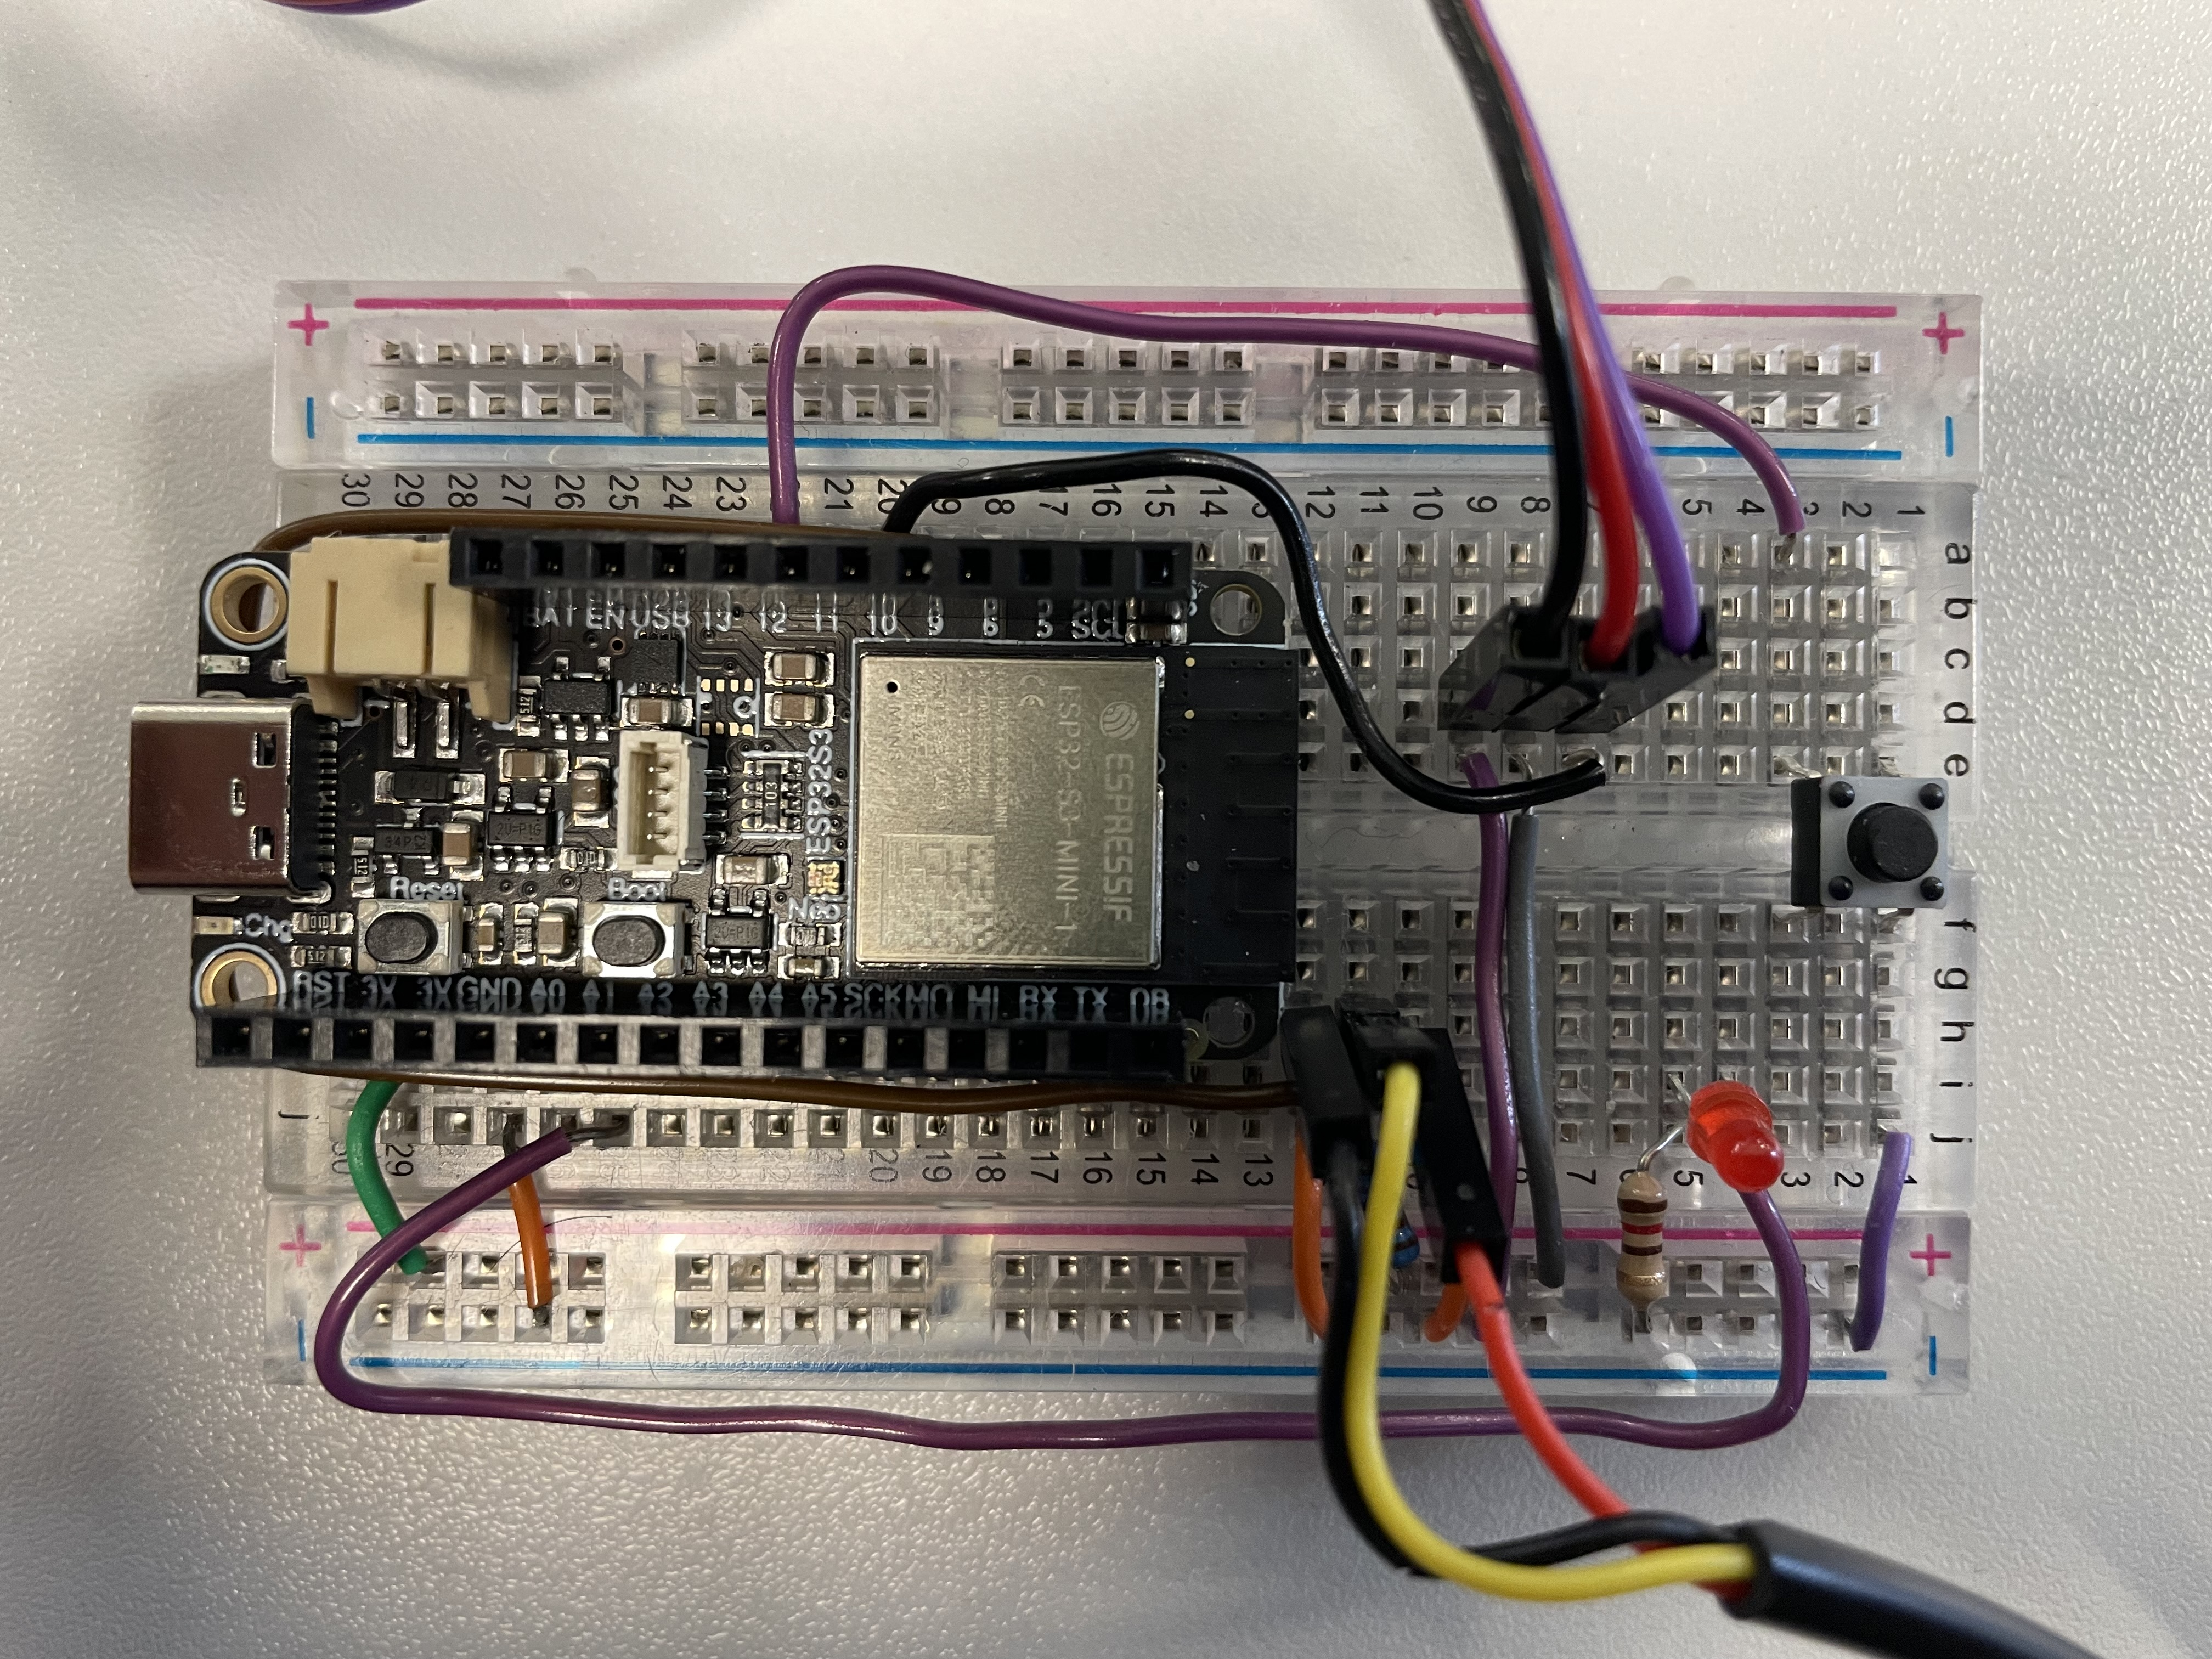
\includegraphics[width=\linewidth]{images/v6-hardware.jpg}
        \caption{Prototype}
        \label{fig:fig-proto}
    \end{subfigure}
    \hfill
    \begin{subfigure}[b]{0.45\linewidth}
        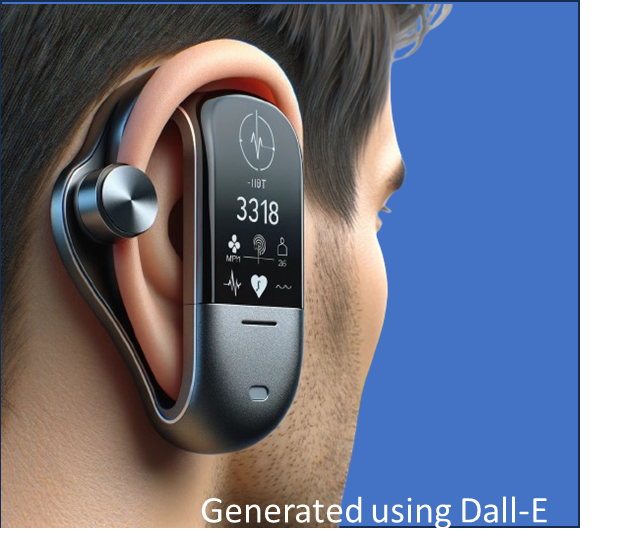
\includegraphics[width=\linewidth]{images/dall-e.png}
        \caption{Design Idea of Physical Product}
        \label{fig:fig-design}
    \end{subfigure}
    \caption{Smart Patch}
    \label{fig:fig-smartpatch}
\end{figure}

\section{Limitations and Issues Encountered}

\subsection{Trade off between Sensor Accuracy and Non-Intrusiveness}
In developing wearable devices for continuous monitoring, a significant challenge is balancing sensor accuracy with the need for non-intrusiveness, particularly for healthcare professionals (HCPs) who wear these devices during long shifts. High accuracy in sensors is crucial, as it ensures that the data collected is reliable enough to inform meaningful interventions to support HCP well-being. However, achieving this often requires more invasive technologies that may interfere with the daily activities and comfort of these professionals.\\ \\
VitalMonitor focuses on optimizing this balance by selecting sensors that minimize intrusiveness while still providing sufficiently accurate data for passive monitoring. This approach is critical in settings where both the well-being of HCPs and operational efficiency are prioritized. Given the limited availability of sensors that strike a perfect balance between non-intrusiveness and high accuracy, the selection was guided by the goal of maintaining user comfort and system reliability. This ensures that healthcare administrators can effectively monitor and respond to the health indicators of their staff without causing discomfort or disruption to their work.


\subsection{Converting Raw Data to Useful Data}

The DS18B20 Temperature Sensor and Pimoroni Pulse Sensor are integral to VitalMonitor's functionality, changing analog electrical signals into digital data for health monitoring. However, this reading process often introduces significant noise, resulting in irregular and unreliable data outputs.  Such anomalies, if unaddressed, could potentially trigger unwarranted alarms or actions based on incorrect information. This necessitates robust data processing strategies to ensure accuracy and usability. \\ \\
A common challenge in sensor data analysis is managing these irregularities, particularly when they lead to significant deviations from expected patterns. For example, an abrupt spike in temperature readings from 32 degrees Celsius to an erroneous 45 degrees could inadvertently exceed the system’s threshold of 35 degrees, resulting in false alarms. To ensure data integrity and reliability, it is imperative to employ robust data smoothing techniques. \\ \\
The Moving Average filter is one such technique applied within the VitalMonitor framework. By averaging data points over a defined time window, this method effectively dampens the impact of transient spikes or noise, leading to a more stable and accurate data output. This technique not only enhances the overall quality of the health monitoring data but also supports critical decision-making processes by reducing the likelihood of false alerts. Figure \ref{fig:data-sensors} provides a snapshot of data collected from the sensors in their raw form as well as data after implementing Moving Average function to it. \\

\begin{figure}[h!]
    \centering
    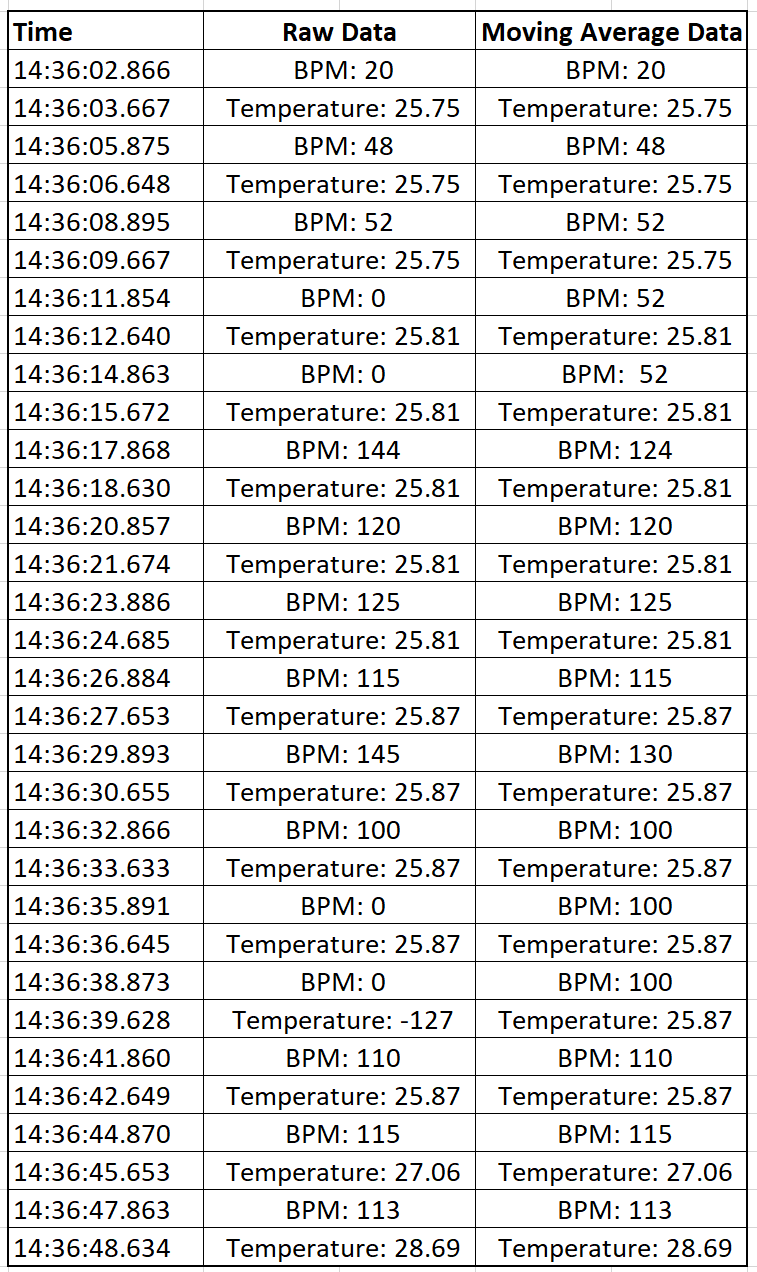
\includegraphics[width=0.6\linewidth]{images/data.png}
    \caption{Data from sensors}
    \label{fig:data-sensors}
\end{figure}

\noindent Extensive testing and evaluation have confirmed that the adapted sensors provide a data precision of \(\pm 15\) BPM for heart rate and \(\pm 0.2-0.5\) degree Celsius for temperature. These measures ensure that VitalMonitor delivers reliable and actionable health data for healthcare professionals, enhancing the monitoring and management of their well-being.

\subsection{Reliability depends on Network Bandwidth}
The effective operation of VitalMonitor’s Smart Patches heavily relies on the strength and capacity of the WiFi network to which they are connected. These devices are designed to upload data in real-time, a process that demands robust network performance to function seamlessly. With a scenario involving up to 100 Smart Patches transmitting data simultaneously, the bandwidth requirements become substantial. This substantial demand can strain the network, leading to potential data transmission delays that may impact the timeliness and reliability of data being displayed on the monitoring dashboard. \\ \\
During extensive testing and evaluation, it was observed that the system's reliability is significantly influenced by the WiFi network's bandwidth. Insufficient bandwidth can result in lagging data updates, which may hinder the system’s ability to provide real-time insights crucial for immediate decision-making and response. This finding underscores the necessity for implementing a network infrastructure capable of supporting high data loads, especially in environments where continuous and simultaneous monitoring is critical. Efforts to enhance network configurations, possibly through dedicated channels or enhanced WiFi protocols, are essential to mitigate these issues and ensure reliable system performance.

\subsection{Google Cloud}
Google Cloud offers \$300 in credits for database and server usage. In this project iteration, these credits were primarily utilized for the MySQL database, specifically the Enterprise Cloud SQL Edition. The chosen configuration, as depicted in Figure \ref{fig:cloud-configurations}, was optimized for cost efficiency, with an initial setup cost of \$6 and a daily operational cost of \$0.4. While suitable for development and testing purposes, this configuration may prove inadequate for production deployment, particularly when supporting a larger user base. \\

\begin{figure}[h!]
    \centering
    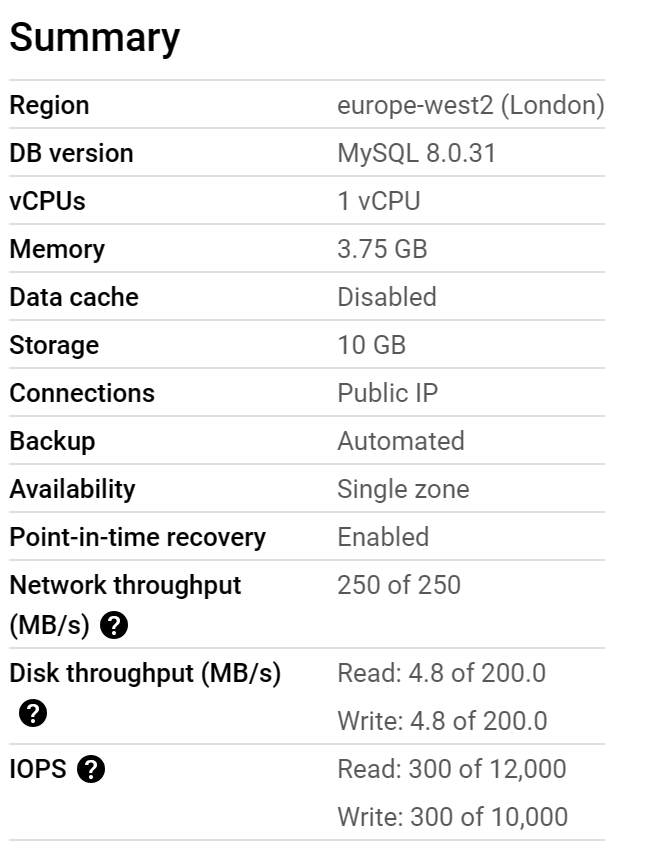
\includegraphics[width=0.5\linewidth]{images/cloud-configurations.png}
    \caption{Google Cloud Configurations}
    \label{fig:cloud-configurations}
\end{figure}

\noindent In a production environment scenario accommodating 100 HCPs and a single dashboard for hospital, upgrading database to the Enterprise Plus Cloud SQL Edition becomes imperative. This entails provisioning a minimum of 8 virtual CPUs, 32 GB of RAM, and increasing storage capacity to over 100 GB. Additionally, as the platform scales to serve multiple hospitals, resource requirements will escalate accordingly.\\

\noindent Furthermore, the middleware microservices will be deployed on Google Cloud in the production phase. These services interact with the database through HTTPS requests, utilizing unix-sockets with appropriate permissions. For instance, when an administrator adds a new device via the dashboard, the workflow involves traversing through the web page, web server, middleware, and database (hosted on Google Cloud) before returning. While deploying middleware on Google Cloud can streamline transactions and improve response times, it necessitates additional costs. Hence, this optimization was deferred in the current iteration to maintain cost-effectiveness.


\section{Further Work}
Despite having achieved the core objectives and beyond, there are more enhancements that this project could have done if not for the time constraint and knowledge-specific constraint. Further Work are divided into 3, things to be done to create a minimum viable product, improving current implementations and finally adding new requirements to make VitalMonitor more efficient.

\subsection{Smart Patch: Final Product}
The culmination of the Smart Patch project will yield a refined, compact device designed to discreetly rest behind the ear. This final iteration will feature optimized sensor placement, with the pulse sensor delicately positioned on the earlobe and the temperature sensor situated inconspicuously behind the ear. Transitioning from the current breadboard prototype to a fully soldered device will be pivotal, streamlining the product for mass production and enhancing its durability.

\noindent To achieve this, future efforts will focus on miniaturizing the device through advanced CAD design and employing more efficient microchips tailored specifically for the Smart Patch. However, before deployment, rigorous testing, including Electrical Safety Testing and Mechanical/Physical Testing, will be necessary to ensure compliance with industry standards and user safety. Although these tests were not feasible within the project's constraints, they remain critical future steps to validate the device's reliability and regulatory compliance.

% The final device will be made in such a way that it sits behind the ear - where the pulse sensor will be sticked to the ear lobe and the temperature sensor right behind the ear. This prototype can be further made more smaller in size using more efficient chips which are streamlined only for Smart Patch unlike ESP32S3. 

% The prototype will be changed from being on the breadboard to a fully soldered device. 

% Further research and design will be done to minituarise the device on CAD. 

% These can be seen in Figure \ref{fig:fig-design}.

% But to even use it on the person a lot of device testing will be involved such as Electrical Safety Testing, Mechanical/Physical Testing. 

% This stage didn't do this because it needs much more Electronics knowledge to conduct such testing and due to time constraints I could have not planned it to finish it in this stage. If given more time, I would have delved into this. 

\subsection{Improving the Middleware Infrastructure}
Current Middleware Infrastructure is implemented as one single webserver but in a way that can be easily divided into 4 microservices (on 4 different web servers) and they all collectively will be known as Middleware. These 4 microservices shall be: Session Management Service, User and Device Management Service, Data Ingestion Service and Data Retrieval Service. Isolating these services and have dedicated server to only take care of one thing - this would reduce the burden on one single web server. This along with a load balancer to keep a queue of request to these servers would help streamline the data, making sure no data is lost. This would not only provide separation of concerns and manage requests but would really help in terms of scalability of the system. 

\subsection{Algorithm to Measure Stress and Fatigue Levels}
As discussed in Chapter 2 Literature Review, that there is no defined way of measuring someone's stress or fatigueness in real-time. Because stress and fatigue are so versatile and depends on so many different factors such as physiological and psychological. Further research can be done to use different vitals and personal information to create an algorithm which can measure this in a numerical form rather than just saying ``the person is feeling 'very' stressed". 

Creating this algorithm would involve a lot inputs from medical researches - in order to best evaluate the reasoning and give weights to certain parameters to accurately define a quantitative way to measure stress and fatigue levels. Once this is defined this would just make so much more quicker for decision making. Of course this would involve a lot more data gathering about HCPs but it would reduce the naive approach based on just thresholds on vitals. 

\subsection{Interdisciplinary Collaboration for Enhanced Sensors}
Like previously discussed about the trade off between sensor accuracy and non-intrusiveness. Interdisciplinary collaboration shall be done with electric engineers, bio-medical engineers to develop enhanced sensors which can not only accurately sense the vitals like heart rate and body temperature, SpO2 and salt intensity in sweats but is also non-intrusive to wear. This would pave a path and make a disruption in the healthcare industry. As much as HCPs want it, patients would also like a non-intrusive way of getting medical treatments. This would enhance their overall experience of getting medical treatments - and would make them less suffer in their sufferings already. 


\subsection{Prediction Model}
Stress and Fatigue are not somethings which usually spikes out. Usually there is gradual growth in their levels except for some cases in stress which can spike out when things go sideways out of nowhere or when you hear a very bad news. But usually, one case see the gradual incline or decline. In the future iterations, a prediction model trained of actual human data which can predict before the stress levels go beyond a control line or threshold. This can give warning signals to the admins of the healthcare organization to better prepare for it rather than once the threshold is crossed only then provide the help. This would provide more time to the admin staff to make arrangements. 

Such a model can either be on the middleware predicting in real-time or it can also be on the firmware or a combination of both.  


